Os materiais utilizados para o experimento foram: goniômetro, lâmpadas de diferentes elementos químicos, lupa e prisma de numeração 17.

para  o início da coleta de dados, o primeiro passo se resumiu a calibrar o goniômetro. Para tal, o prisma foi retirado do goniômetro, a luneta de leitura foi destravada e alinhada com com a entrada de luz da lâmpada de Sódio, travando a luneta. Na sequência, o foco da luneta foi ajustado de para que a cruz no interior da mesma pudesse ser visto de forma nítida, assim como a fenda de entrada de luz; o parafuso de ajuste fino foi empregado para garantir que a cruz se alinhasse com o lado fixo da fenda. Para finalizar o ajuste, o disco graduado do goniômetro foi liberado seu "zero" foi alinhado com o "zero" da luneta.

Para próxima etapa do experimento, foi preciso determinar o ângulo $\alpha$ do ápice do prisma, isto é, a separação angular entre as duas faces do prisma mais próximas à fonte de luz. Para isto, considerou-se os dois raios luz $L_1$ e $L_2$ refletidos pelas faces do prisma, e o resultado geométrico que mostra que $\Delta \theta_L = \theta_{L_1} + \ang{360} - \theta_{L_2} = 2 \alpha$, ou seja, a separação angular entre os raios é igual ao dobro do ápice, como ilustrado abaixo.

\begin{figure}[H]
	\centering	    
	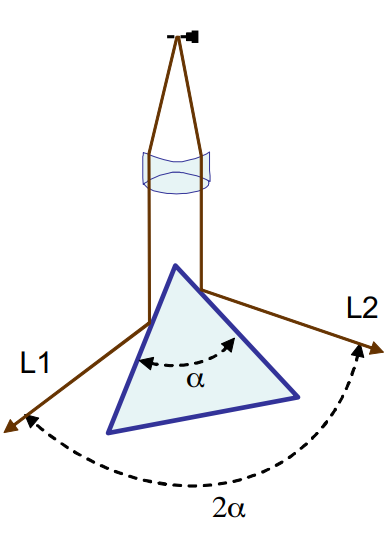
\includegraphics[scale=0.30]{figuras/alpha.png}
	\caption{Diagrama para a obtenção de $\alpha$}
	\label{fig:alpha}
\end{figure}

Com o ápice do prisma devidamente determinado, a fim de determinar o coeficientes $A$ e $B$ da equação de Cauchy com dois termos, indicada como uma aproximação apropriada no espectro de luz visível~\cite{ref:otica}:
\begin{equation}
    n(\lambda) = A + \frac{B}{\lambda^2}
    \label{eq:cauchy}
\end{equation}
Mostrando-se necessário coletar dados para o ângulo de desvio mínimo $\delta_\text{min}$ das raias espectrais de dispersão e determinar o índice de refração através da relação:

\begin{equation}
    n\left(\delta_\text{min}\right) = \frac{
        \sin\left(\frac{\alpha + \delta_\text{min}}{2}\right)
    }{
        \sin\left(\frac{\alpha}{2}\right)
    }
    \label{eq:n}
\end{equation}

 Assim, possibilitando a construção de um gráfico de $n$ por $1/\lambda^2$ em que $A$ e $B$ equivalem, respectivamente, aos coeficientes linear e angular do ajuste.

Para determinação dos desvios mínimos de cada raia espectral, lâmpadas baseadas em diferentes elementos químicos foram empregadas, no caso, os elementos utilizados foram: Sódio, Mercúrio, Cádmio e Hélio. O procedimento experimental consistia da observação das raias espectrais mais intensas geradas a partir da luz emitida pelas lâmpadas, de forma que o ângulo mínimo de dispersão de cada uma delas fosse medido com auxilio do goniômetro. Na sequência, os comprimentos de onda de cada raia foi obtido a partir de valores tabelados na literatura. Foram coletados dados para as 3 raias mais intensas de cada lâmpada, com exceção do Hélio, em que 4 raias puderam ser observadas com clareza.

Por fim, com os dados coletados, foi possível determinar os coeficiente $A$ e $B$ e por fim, utilizando a equação \ref{eq:n} e seguinte inversão da equação de Cauchy:
\begin{equation}
    \lambda = \sqrt{\frac{B}{n\left(\delta_\text{min}\right)-A}}
    \label{eq:lambda}
\end{equation}
foi gerada um curva que pode ser empregada como espectrômetro.


\subsection{Incertezas associadas}

O único tipo de medição experimental coletado diretamente foi o de ângulos, para os quais as resolução da medida era $\text{res}=\ang{;1;}$. Com base nisso, foram atríbuidas duas incertezas, a incerteza da leitura, que segue uma distribuição triangular de $\pm\text{res}/2$, e a incerteza de paralaxe do posicionamento na leitura, que poderia mover o encaixe dos minutos para as posições adjacentes, que foi calculada com uma distribuição retangular de $\pm\text{res}$. Isso nos leva a incerteza acumulada da medida, que foi feita com base nas recomendações do GUM\cite{ref:gum}.

\begin{gather*}
    u_{\text{leitura}} = \frac{\text{res}}{2 \sqrt{6}} = \text{res} \frac{\sqrt{6}}{12} \\
    u_{\text{paralaxe}} = \frac{2\ \text{res}}{2 \sqrt{3}} = \text{res} \frac{\sqrt{3}}{3} \\
    \Delta{\delta_{\text{min}}} = \Delta\theta_L = u_{\text{medida}}
        = \sqrt{u_{\text{leitura}}^2 + u_{\text{paralaxe}}^2}
        = \text{res} \frac{\sqrt{6}}{4}
\end{gather*}

Todos os outros valores, calculados as partir desses ângulos e de valores referenciados de outros trabalhos, tiveram suas incertezas encontradas por meio da propagação das incertezas inicias. Como é o caso da equação de incerteza abaixo, alcançada pela eq. teórica do $\alpha$, que veio diretamente da figura \ref{fig:alpha}.

\begin{equation*}
    \Delta{\alpha} = \sqrt{{\Delta{\text{L}_1}}^2\frac{1}{4} + {\Delta{\text{L}_2}}^2\frac{1}{4}} = \Delta\theta_L \frac{\sqrt{2}}{2}
\end{equation*}

O mesmo foi feito para a equação do índice de refração (\ref{eq:n}), como segue abaixo:

\begin{align*}
    \Delta{n} &= \sqrt{
        \Delta{\alpha}^2 \left(\frac{\partial n}{\partial\alpha}\right)^2
        + \Delta{\delta^2_{\text{min}}} \left(\frac{\partial n}{\partial\delta_{\text{min}}}\right)^2
    } \\
    &= \frac{1}{2} \sqrt{
        \Delta{\alpha}^2 \frac{\sin^2(\delta_{\text{min}}/2)}{\sin^4({\alpha/2})}
        + \Delta{\delta^2_{\text{min}}} \frac{\cos(\alpha+\delta_{\text{min}})+1}{1-\cos(\alpha)}
    }
\end{align*}

A equação de incerteza mais importante aqui talvez seja a eq. \ref{eq:u:lambda}, abaixo, que é usada para analisar a resolução final do equipamento.

\begin{equation}
    \Delta{\lambda} = \sqrt{
        \Delta{A}^2 \left(\frac{\partial\lambda}{\partial A}\right)^2
        + \Delta{B}^2 \left(\frac{\partial\lambda}{\partial B}\right)^2
        + \Delta{\alpha}^2 \left(\frac{\partial\lambda}{\partial\alpha}\right)^2
        + \Delta{\delta^2_{\text{min}}} \left(\frac{\partial\lambda}{\partial \delta_{\text{min}}}\right)^2
    }
    \label{eq:u:lambda}
\end{equation}

Tendo em mente que $n(\delta_\text{min})$ se refere a eq. \ref{eq:n}, os fatores da eq. \ref{eq:u:lambda} são os dados abaixo:

\begin{gather*}
    \left(\frac{\partial\lambda}{\partial A}\right)^2 = \frac{B}{4 (n(\delta_\text{min})-A)^3} \\
    \left(\frac{\partial\lambda}{\partial B}\right)^2 = \frac{1}{4 B (n(\delta_\text{min})-A)} \\
    \left(\frac{\partial\lambda}{\partial\alpha}\right)^2 = \frac{B}{16 (n(\delta_\text{min})-A)^3} \frac{\sin^2(\delta_\text{min}/2)}{\sin^4(\alpha/2)}\\
    \left(\frac{\partial\lambda}{\partial\delta_\text{min}}\right)^2 = \frac{B}{16 (n(\delta_\text{min})-A)^3} \frac{\cos(\alpha+\delta_\text{min})+1}{1-\cos(\alpha)}
\end{gather*}

No caso das incertezas de $A$ e $B$, o seu valor foi extraído pelo modelo de regressão linear por mínimos quadrados, como descrito no final do Guia de Incertezas~\cite{ref:gum}, bem como os valores utilizados para esses parâmetros. A única exceção sobre a incerteza dos valores é com os comprimentos de onda $\lambda$ que foram retirados da referência usada como base do experimento~\cite{ref:roteiro}, e, portanto, não possuem incertezas associadas.
